\section{Добавление аккуаунта эл.почты}
Для добавления аккаунта эл.почты необходимо выполнить следующие:
\begin{enumerate}[\thesection .1]
\item  Зайти в меню планшета (рис.\ref{pic:pic_1}):
 \begin{figure}[H]
 	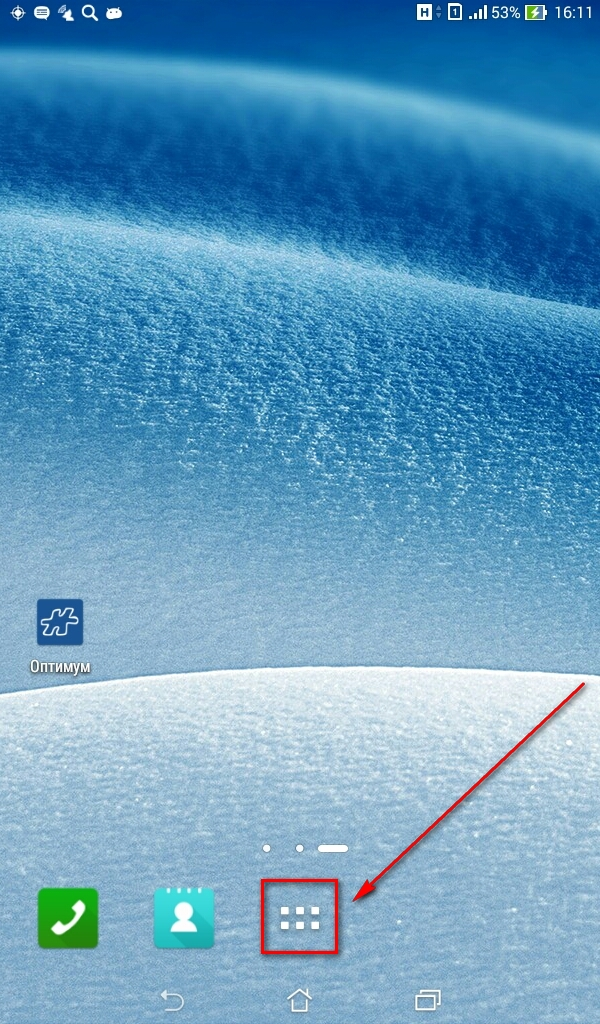
\includegraphics[width=0.3\linewidth]{pic_1.jpg} 
 	\caption{Меню}\label{pic:pic_1}
 \end{figure}
\item Выбрать и нажать на значок "Настройка" планшета (рис.\ref{pic:pic_2}):
 \begin{figure}[H]
 	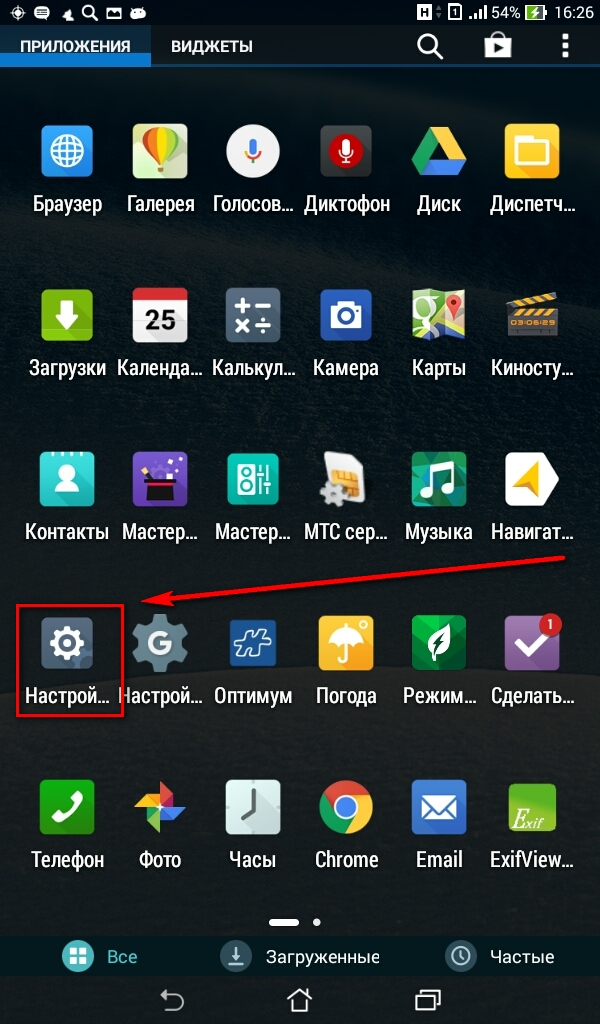
\includegraphics[width=0.3\linewidth]{pic_2.jpg} 
 	\caption{Настройка}\label{pic:pic_2}
 \end{figure}
\item Откроется окно настроек планшета (рис.\ref{pic:pic_3}):
 \begin{figure}[H]
 	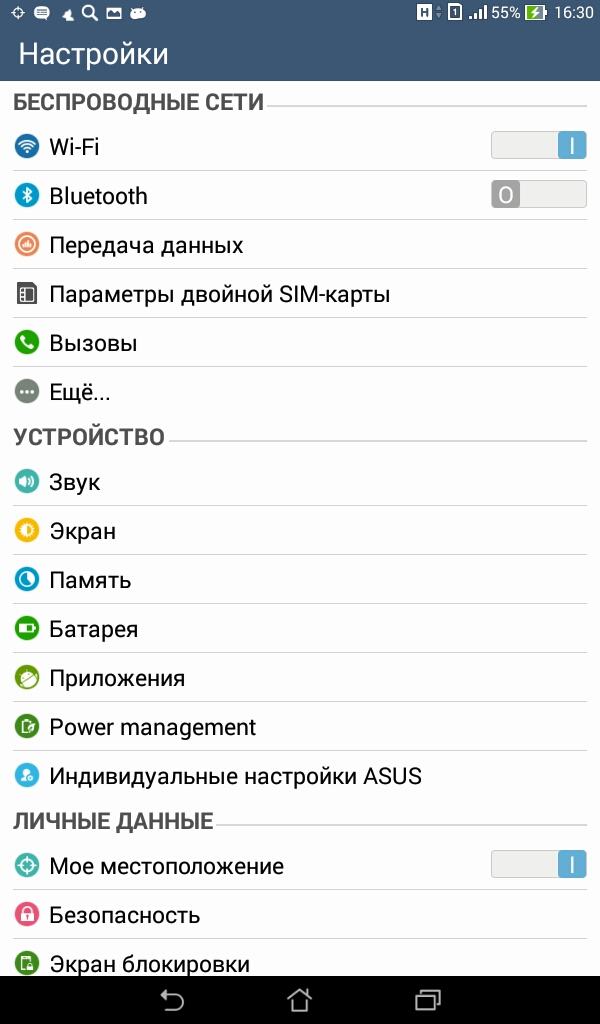
\includegraphics[width=0.3\linewidth]{pic_3.jpg} 
 	\caption{Настройки планшета}\label{pic:pic_3}
 \end{figure}
 \item "Пролистать" список вниз до появления пункта "Добавить аккаунт" (рис.\ref{pic:pic_4}):
  \begin{figure}[H]
  	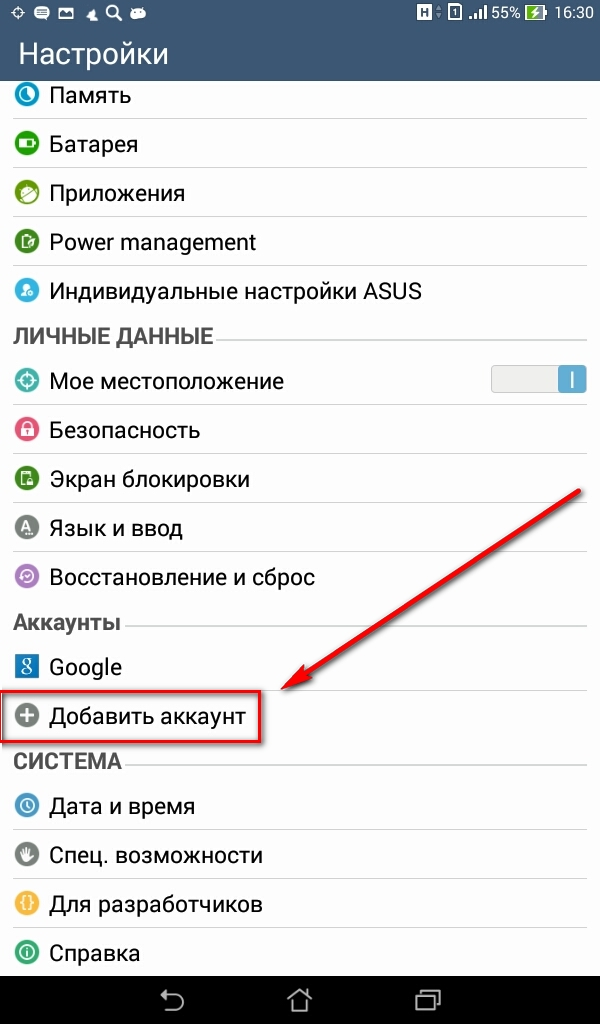
\includegraphics[width=0.3\linewidth]{pic_4.jpg} 
  	\caption{Пункт "Добавить аккаунт"}\label{pic:pic_4}
  \end{figure}
\item Выбрать его, затем найти и выбрать "Google" (рис.\ref{pic:pic_5}):
  \begin{figure}[H]
  	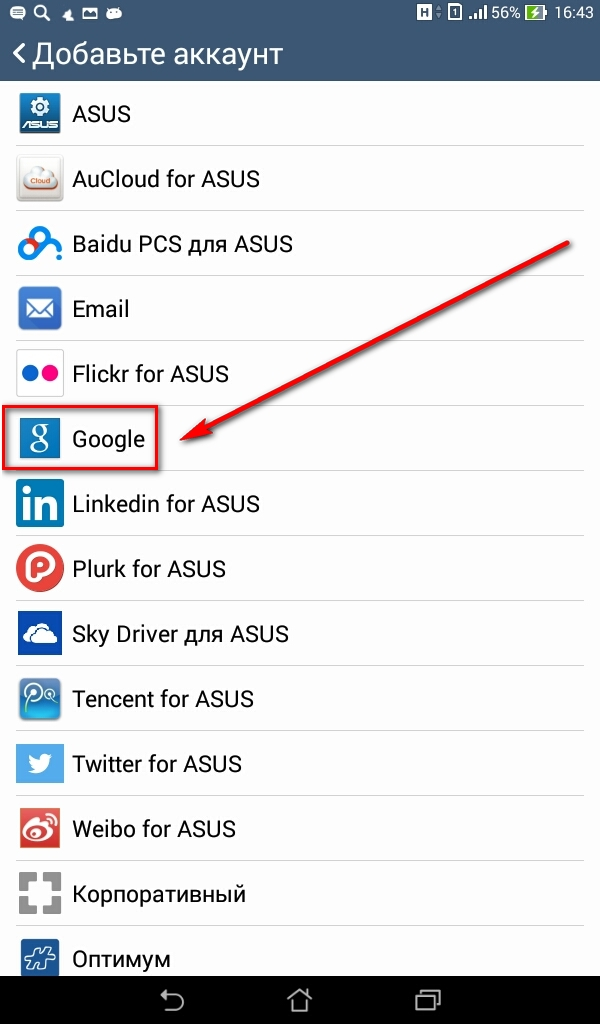
\includegraphics[width=0.3\linewidth]{pic_5.jpg} 
  	\caption{"Google"}\label{pic:pic_5}
  \end{figure}
  
\begin{itemize}[topsep=0pt, itemsep=-0.5ex]
	\item сбор дебиторской задолженности у клиентов
	\item поиск новых клиентов
	\item экстренной ситуации, требующей незамедлительного присутствия торгового представителя.
\end{itemize}
\item Торговый представитель может принимать заявки по телефону от торговых точек, не указанных в маршрутном листе соответствующего рабочего дня.
%\item Рабочий день торгового представителя (согласно данным GPRS), а именно, посещение последней торговой точки согласно маршрутному листу, заканчивается в 16:30.
\end{enumerate}